
\section{Overview}
\label{sec:overview}


According to the task given in the manual, a general purpose processor implementing the ARM Thumb-2 has been designed. All operations specified in this architecture, except \texttt{CBNZ} and \texttt{CBZ}, and operations on processor state change, are implemented. Both the \texttt{count32} and the \texttt{memcp46} benchmark applications can be executed.

The processor consists of the following larger submodules, as pointed out in Fig. \ref{fig:processorOverview}:
\begin{itemize}
\itemsep-1em 
\item Instruction Decoder
\item Register File
\item Instruction Fetch Unit
\item ALU (purely combinatorial)
\item Flag Updater (purely combinatorial)
\item Memory Interface
\end{itemize}

\subsection{Pipeline Stages}
There are two pipeline stages: one pipeline register is at the decoder output, the other at the output of the register file. In short, the stages could be called \textit{fetch/decode} and \textit{execute/writeback}.

\subsection{Control}
The whole processor is controlled by the decoder. This decision has been taken since we encountered that the most control decisions depend on complex instructions.

\subsection{Memory Access}
All memory access are abstracted from the rest of the CPU through a dedicated memory interface. This interface registers simple read/write request signals and executes the memory access. Addresses in the THUMB architecture are byte aligned, but the memory is halfword aligned. Therefore, the conversion of the requested address to the required address (-es) is performed by this module Additionally, sign extensions can be done on the data output.

\subsection{ALU and Flags}
All arithmetic operations are executed by a combinatorial ALU. It also outputs the values for the required flags (C, V, Z, N). The flags are only updated by a flag updater if the instruction requires that.

\subsection{Instruction Decoder}
The Instruction Decoder outputs all control signals one cycle after the instruction has been assigned. Furthermore, it has a state machine which manages the control signals in the following cycles.If necessary (at memory or multi-instructions), it may stall the instruction fetch. 

\subsection{Register File}
The register file features four read- and 2 write ports. Additionally, it has separate outputs for the PC and the status flag register.

\subsection{Instruction Fetch}
Instructions are loaded from the memory by the instruction fetch. It also updates the PC if no stall or branch is applied.


\begin{figure}
%\centering
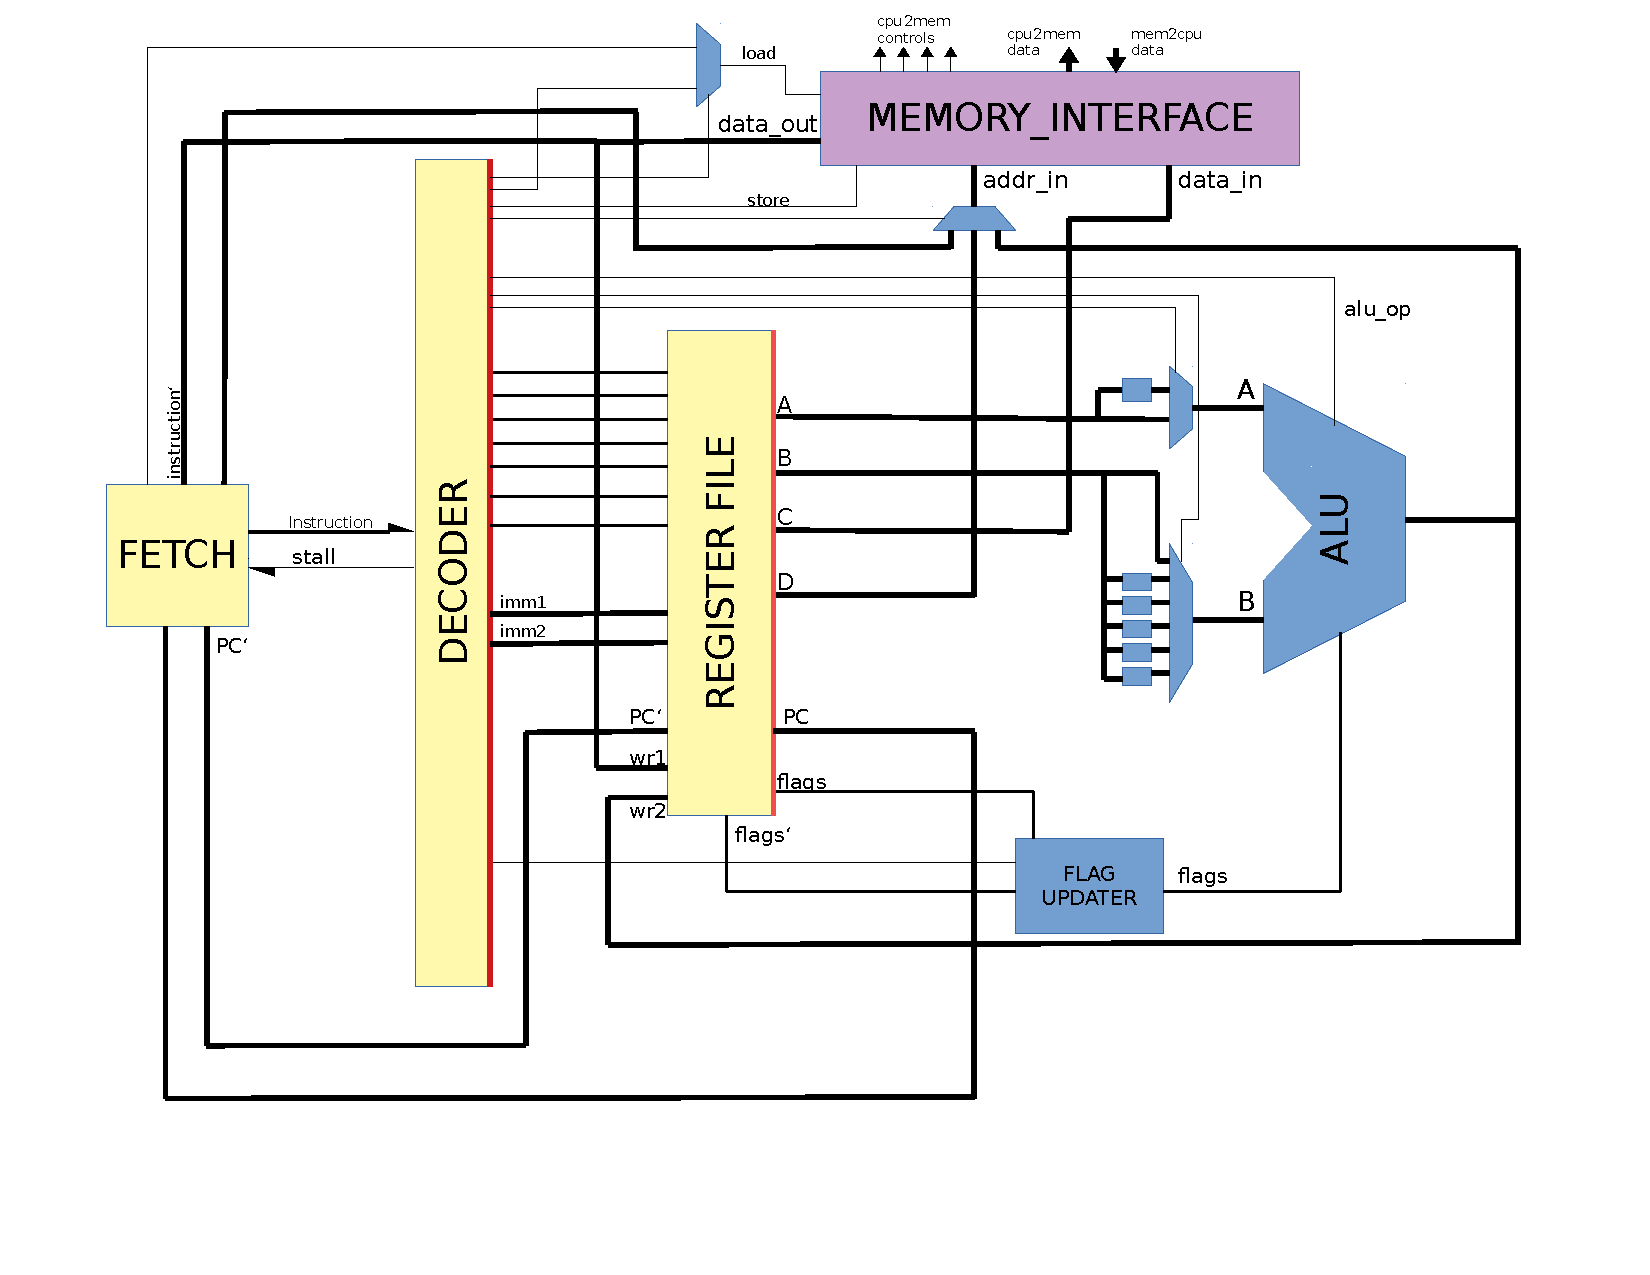
\includegraphics[scale=0.65]{images/processorOverview}
\caption{Overview of the designed micro-architecture. Pipeline registers are marked red.}
\label{fig:processorOverview}
\end{figure}

\section{Performance}

The performance of the designed processor is shown in table \ref{tab:performance}.

\centering
\begin{tabular}{|c|c|c|c|c|c|c|}
\hline 
Type & Clock Period & max. Frequency & \#Cycles/count32 & \#Cycles/memcp46
& Area & Power \\ 
\hline 
Value & 1 ns & 2 GHz & 300 & 400 & 300 qm & 5 GW \\ 
\hline 
\end{tabular} 
\label{tab:performance}
